\documentclass{beamer}
\usetheme{Madrid}
\usepackage{amsmath}
\usepackage[utf8]{inputenc}
\title{Tax Saliency}
\author{by Xiaomin Li}
\centering
\date{September 2019}
\begin{document}
\maketitle
\begin{frame}{Content}
\begin{itemize}
\item Taubinsky Rees-Jones, 2017 
\end{itemize}
\end{frame}
\begin{frame}{Taubinsky Rees-Jones, 2017}
\framesubtitle{Summaries}
\begin{itemize}
    \item Consumers under-react to non-salient tax on average
    \item Heterogeneity increases the efficiency cost of taxation
    \item Counting for this endogeneity increases efficiency cost
\end{itemize}
\end{frame}
\begin{frame}{Set-up}
   \begin{itemize}
       \item Total utility: $u(y)+vx$,
       \\$x \in \{0,1\}$, $v$ is the value of the product,y is remaining income
       \\$x=1$ iff $u(Z-p-t)+v \ge u(Z)$
       \item Inattentive setting: $u(Z-p-\theta t)+v\ge u(Z)$
       \\$\theta$ denotes the level of under/over reacts to tax 
       \item In this paper, $\theta := \frac{p_{max} (0)-p_{max} (t)}{t}$
       \item Elasticity to tax: $\epsilon_{D,t}(p,t)=-D_t(p,t)\frac{p+t}{D(p,t)}$
       \\$D_t(p,t)$ is the partial derivative of tax on demand
\end{itemize}
\end{frame}

\begin{frame}{Direct efficiency costs to tax}

\[
    \frac{d}{dt}EB(t,F_t) = -E[\theta|p,t]t \frac{d}{dt} D(p(t),t)-Var[\theta|p,t]tD_p(p(t),t)\]
   
  \[=E[\theta|p,t]tD(p(t),t)\frac{\epsilon^{TOT}_{D,t}}{p(t)+t}
+\frac{Var[\theta|p,t]}{E[\theta|p,t]}tD(p(t),t)\frac{\epsilon_{D,t}}{p(t)+t}
\]
  \begin{itemize}
      \item $Ft(v,\theta)$ is the distribution of value and $\theta$
      \item $E[\theta|p,t]$ and $Var[\theta|p,t]$ are mean and variance of $\theta$ for those who are indifferent about purchasing at $p,t$
      \item $\epsilon^{TOT}_{D,t}$ is the elasticity of tax on demand at equilibrium.
  \end{itemize}
\end{frame}
\begin{frame}
\frametitle{Effect of nudge}
 
\begin{block}{Prep 5 in paper}
Two taxes $t_1$ and $t_2=t_1+\Delta t$. Producer prices are fixed. Assumption A-C satisfied (Very mathy assumptions not important).
\end{block}
 
\[
EB(t_2,F_{t_2}) -EB(t_1,F_{t_1})=\]\\
\[ -(t_1(\Delta t)+\frac{(\Delta t)^2}{2})(E[\theta|p,t_2]^2+Var[\theta|p,t_2])D_p -\frac{(t_1^2}{2}(E[\theta^2|p,t_2]-E[\theta^2|p,t_1])
\]
\end{frame}
\begin{frame}
\frametitle{Identification}
\begin{block}{Representative Agent case}
$\theta$ can be identified by $D_t(p,t)/D_p(p,t)$. This is from CLK
\end{block}
\begin{block}{Heterogeneous inattentiveness}

\end{block}
\end{frame}
\begin{frame}
   \frametitle{Experiment Design}
   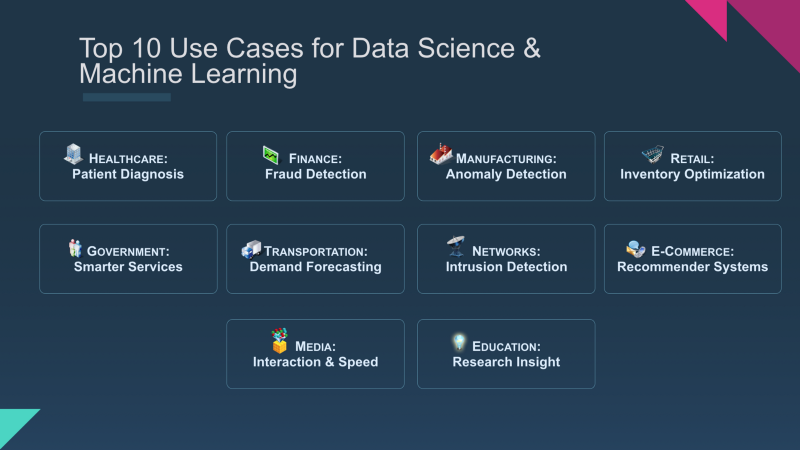
\includegraphics[height=6.8cm]{1_kTnSJQpzGw_w4uQKa_j7VQ.png}
\centering
\end{frame}

\begin{frame}{Classification: Applications}
    \begin{itemize}
        \item Aka Pattern recognition
\item Face recognition: Pose, lighting, occlusion (glasses, beard), make-up, hair style 
\item Character recognition: Different handwriting styles.
\item Speech recognition: Temporal dependency. 
\item Use of a dictionary or the syntax of the language. 
\item Sensor fusion: Combine multiple modalities; eg, visual (lip image) and acoustic for speech
\item Medical diagnosis: From symptoms to illnesses
\item Web Advertizing: Predict if a user clicks on an ad on the Internet.
\end{itemize}
\end{frame}

\begin{frame}{Main Application}
    \begin{itemize}
        \item Face Recognition
        \item Prediction: Regression
        \item Regression Applications
    \end{itemize}
\end{frame}

\begin{frame}{Top 10 use cases of Machine Learning}

\end{frame}

\begin{frame}{What machine learning tools do Kaggle champions use?}
 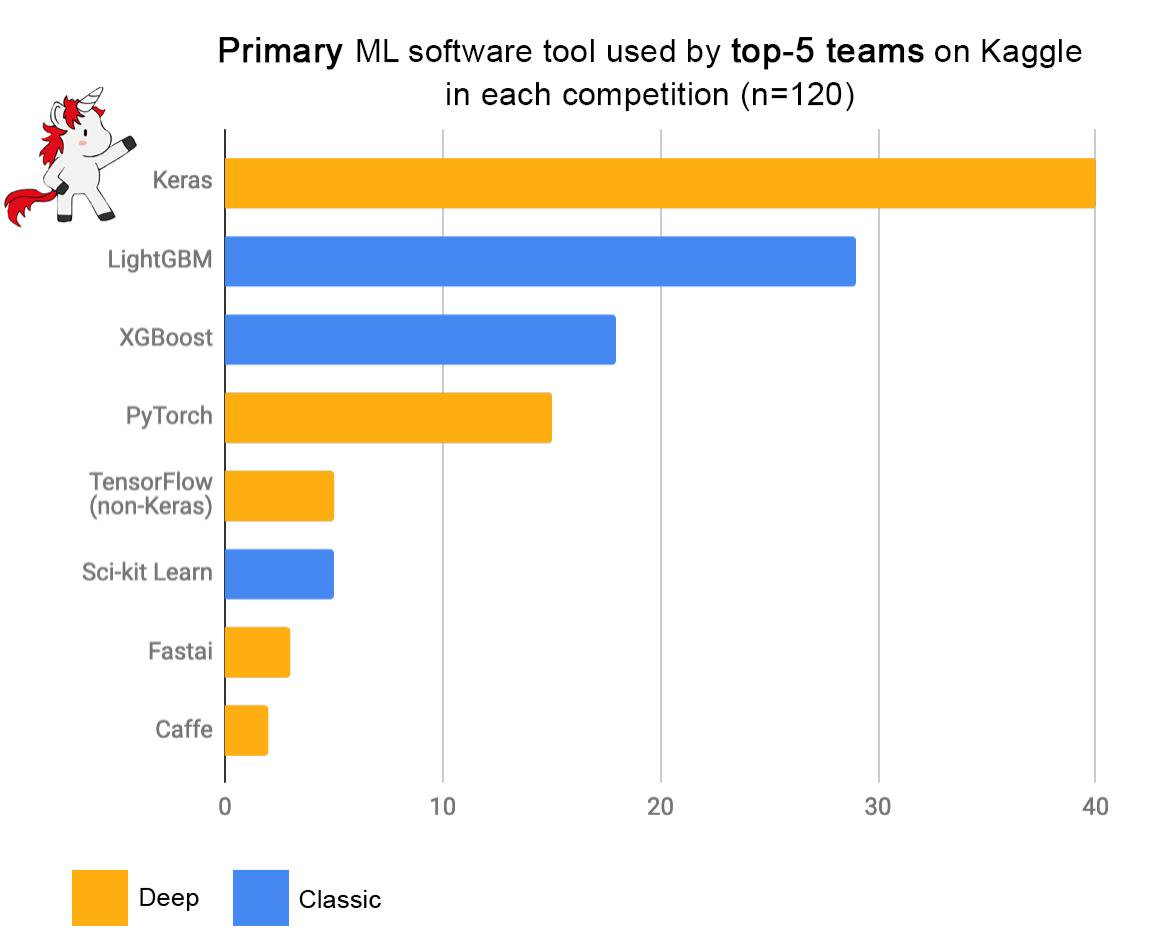
\includegraphics[height=6.8cm]{D3Pb_Q3UIAAuSWU.jpg}
\centering   
\end{frame}

\begin{frame}{Types of Learning?}
\begin{itemize}
    \item Supervised Learning: Uses
    \item Unsupervised Learning
    \item Reinforcement Learning
\end{itemize}
\end{frame}

\begin{frame}{Supervised Learning: Uses}
   \begin{block}{Prediction of future cases}
   Use the rule to predict the output for future inputs
   \end{block}
   \begin{block}{Knowledge extraction}
 The rule is easy to understand
   \end{block}
   \begin{block}{Compression}
  The rule is simpler than the data it explains
   \end{block}
   \begin{block}{Outlier detection}
   Exceptions that are not covered by the rule, e.g., fraud
   \end{block}
  
\end{frame}

\begin{frame}{Unsupervised Learning}
    \begin{itemize}
        \item Learning “what normally happens”
\item No output
\item Clustering: Grouping similar instances
\item Other applications: Summarization, Association Analysis. \end{itemize}
\begin{block}{Example applications}
\begin{itemize}
    \item Customer segmentation in CRM
\item Image compression: Color quantization
\item Bioinformatics: Learning motifs
\end{itemize}
\end{block}
\end{frame}

\begin{frame}{Reinforcement Learning}
    \begin{itemize}
        \item No supervised output but delayed reward
        \item Policies: what actions should an agent take in a particular situation.Utility estimation: how good is a state (used by policy)
        \item Credit assignment problem (what was responsible for the outcome) 
     \end{itemize}
     \begin{block}{Applications}
     \begin{itemize}
        \item Game playing
        \item Robot in a maze
        \item Multiple agents, partial observability, ...
     \end{itemize}
     \end{block}
   \end{frame}

\begin{frame}
\huge{\centerline{The End}}
\end{frame}

\end{document}
